\documentclass{article}
\usepackage{amsmath}
\usepackage{amssymb}
\usepackage{graphicx}
\usepackage{hyperref}
\usepackage[version=4]{mhchem}

\title{Example 8}
\date{}

\begin{document}
\maketitle

(2001 China Middle School Math Contest) As shown in the figure, triangle \(A B C\) and point \(P\) in the same plane are given. \(P A=\) \(P B . \angle A P B=2 \angle A C B\). \(A C\) intersects \(B P\) at point \(D\). If \(P B=4\) and \(P D=3\), then \(A D \cdot C D=\)\\
(A) 6\\
(B) 7\\
(C) 12\\
(D) 16

Solution: (B).\\
\centering
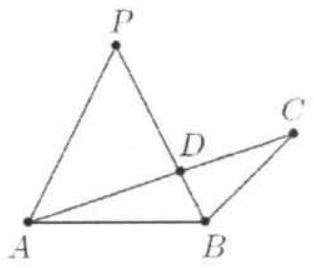
\includegraphics[width=\textwidth]{images/problem_image_1.jpg}

Extend \(B P\) to \(E\) such that \(P E=P B\). Since \(P A=P B=P E\), points \(A, B\), and \(E\) are concyclic. Construct this semicircle with center \(P\) as shown in the figure to the right.\\
So we have \(\angle A E B=\frac{1}{2} \angle A P B=\angle A C B\). We also know that \(\angle A D E=\angle B D C\) (vertical angles). Therefore \(\triangle A E D \sim\) \(\triangle D C B\).\\
\(\frac{A D}{B D}=\frac{E D}{D C} \Rightarrow A D \cdot C D=E D \cdot B D=(P E+P D)(P B-\)\\
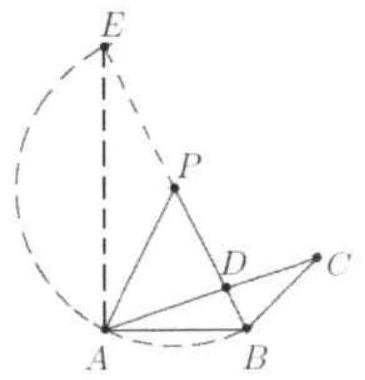
\includegraphics[width=\textwidth]{images/reasoning_image_1.jpg} \(P D)=(4+3)(4-3)=7\).


\end{document}
